\chapter{Metodologia}
\label{chap:MatMet}

O Capítulo \ref{chap:FUNDA} apresentou alguns dos métodos encontrados na literatura para a representação computacional de formas a partir do contorno.  Em muitos casos, esses métodos apresentam parâmetros que requerem ajustes dependentes da natureza da aplicação, ou seja,  das características da base de imagens e o propósito ao qual o sistema de reconhecimento se destina. A energia de dobramento multiescala, por exemplo, requer o ajuste do número e dos valores das escalas utilizadas na representação das formas. 

Esse capítulo apresenta um método robusto e versátil para o ajuste desses parâmetros para customizar descritores multiescala à base de imagens de formas, para fins de melhoria do desempenho em classificação supervisionada e não supervisionada. 

\section{Base de imagens}
Temos na Figura \ref{fig:leaves} exemplares de folhas extraídas da base de imagens Flavia \cite{}.

\begin{figure}[!ht]
\caption{\label{fig:leaves} Trinta e duas amostras extraídas da base Flavia, que contém $1907$ imagens de folhas de $32$ espécies diferentes. Cada amostra corresponde a uma espécie.}
\centering
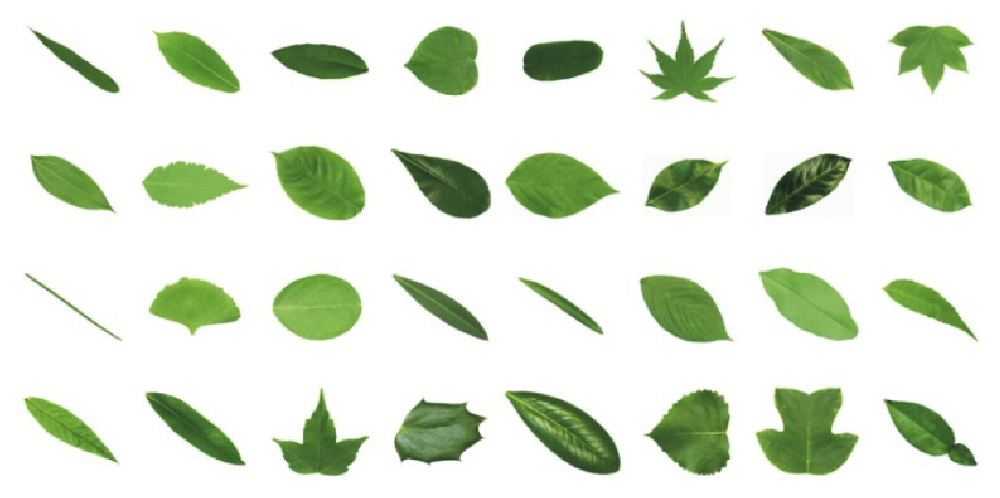
\includegraphics[width= \textwidth]{folhas.eps}
\end{figure}

\section{Extração de atributos}

\subsection{Energia de dobramento multiescala\label{subsec:BE}}

\citeonline{Young:1974} propuseram a energia de dobramento como uma medida de complexidade para análise de formas biológicas. Conceitualmente, esta é definida como sendo a energia necessária para se modificar uma forma, através de deformações, ao seu estado de menor energia, ou seja, um círculo do mesmo perímetro da forma deformada.

A maneira mais direta de se obter a energia de dobramento de um contorno fechado é a partir de sua curvatura pela seguinte expressão:

\begin{equation}\label{eq:be}
E = \frac{1}{L}\int\limits_{l}K^2(l)dl\text{,}
\end{equation}
\noindent
sendo $L$ o perímetro do contorno e a integral calculada ao longo do comprimento de seu arco. O resultado da equação \ref{eq:be} é um escalar que representa a energia média do sinal da curvatura.

\begin{comment}
A energia de dobramento multiescala é obtida a partir da curvatura multiescala repetindo-se o cálculo da equação \ref{eq:be} para diferentes níveis de suavização do contorno. Isso resulta em um vetor de características composto por escalares decorrentes da curvatura multiescala para cada uma das escalas empregadas na suavização do contorno e cálculo da curvatura. 
\end{comment}

A energia de dobramento multiescala foi introduzida por \citeonline{Costa:1997} para a análise de formas de neurônios. Nesta tese investigamos sua utilização como um descritor de propósito geral em recuperação de formas pelo conteúdo. Para um contorno discreto, com $N$ pontos, representado na forma complexa $z[n] = x[n]+jy[n] \text{,} \quad n \quad \epsilon \quad [0, \quad 1, \quad \ldots \quad , \quad N-1]$, a energia de dobramento é dada por: 

\begin{equation}
E_{be} = \frac{L^{2}}{N}\sum_{n=0}^{N-1}K^{2}[n]\text{,}
\label{eq:ebe}
\end{equation}
\noindent
sendo o perímetro do contorno elevado ao quadrado ($L^2$) uma constante de normalização para que o descritor tenha invariância a escala. A curvatura discreta $K[n]$ é calculada a partir de $z[n]$ através da seguinte expressão:

\begin{equation}
K[n] = \frac{-Im(z^{'}[n](z^{''}[n])^{*})}{|z^{'}[n]|^3} \text{,}
\label{eq:kn}
\end{equation}
\noindent
aonde $z^{'}[n]$ e $z^{''}[n]$ correspondem as derivadas primeira e segunda e $z^{*}[n]$ o conjugado de $z[n]$. 

A energia de dobramento multiescala resulta da versão discreta da curvatura multiescala. Podemos calcular as derivadas primeira e segunda do contorno discreto suavizado ($z_\sigma'[n]$ e $z_\sigma''[n]$) através das propriedades da derivada da convolução ou da transformada de Fourier. No caso discreto, a transformada de Fourier de $z[n]$ é dada por:  

\begin{equation}
Z[s] = F\big\{z[n]\big\} = \sum\limits_{n=0}^{N-1}z[n].e^{\frac{-j2\pi ns}{N}} \text{,}
\end{equation}

$s = -N_{2}\: \ldots \: N-N_{2}-1\text{, }N_{2}=floor\big(\frac{N}{2}\big)$.

 A transformada inversa é dada por  

\begin{equation}
z[n] = F^{-1}\big\{Z[s]\big\} = \sum\limits_{s = -N_{2}}^{N-N_{2}-1}Z[s]e^{\frac{j2\pi n s}{N}}\text{,}
\end{equation}
 $ n = 0\: \ldots \: N-1$.
  
No domínio $s$ o contorno é suavizado multiplicando-se, elemento a elemento, $Z[s]$ pela transformada de Fourier da versão discreta do filtro passa baixas gaussiando $g_\sigma[n] = \frac{1}{\sigma\sqrt{2\pi}}e^{\frac{n^2}{2\sigma^2}}\text{, } 
n = 0 \: \ldots \: N-1$:

\begin{equation}
Z_\sigma[s] = Z[s].F\big\{g_\sigma[n]\big\}\text{,}
\end{equation}
\noindent
 sendo as referidas derivadas do contorno suavizado:
\begin{equation}
z_\sigma'[n] = F^{-1}\big\{j2\pi s Z_\sigma[s]\big\}
\end{equation} e
\begin{equation}
z_\sigma''[n] = F^{-1}\big\{-(2\pi s)^2 Z_\sigma[s]\big\}\text{.}
\end{equation}

O processo de filtragem passa-baixas diminui a energia espectral da representação complexa do contorno resultando no encolhimento do seu perímetro. Uma estratégia para compensar tal efeito é normalizar o contorno suavizado com a razão entre o perímetro do contorno não suavizado ($L$) e o seu perímetro ($L_{\sigma}$) \cite{Cesar:1996,Costa:1997}:

\begin{equation}
\breve{z}_{\sigma}[n] = \frac{L}{L_{\sigma}}z_{\sigma}[n]\text{.}
\end{equation}

Substituindo $K[n]$ por $K_{\sigma}[n]$ e $z[n]$ por $\breve{z}_{\sigma}[n]$ nas equações \ref{eq:kn} e \ref{eq:ebe}, e realizando estes cálculos para $M$ escalas distintas $(\sigma_1\text{, }\sigma_2\text{, }\text{, }\ldots\text{, }\sigma_M)$ resulta na representação multiescala da energia de dobramento:

\begin{equation}
NMBE = (\log{E_{\sigma_{1}}}\text{, }\log{E_{\sigma_{2}}}\text{, }\ldots \text{ , }\log{E_{\sigma_{M}}})\text{.}
\label{eq:nmbe}
\end{equation}

\section{Função custo e otimização}
A metodologia para escolha de parâmetros do descritor segue o esquema da Figura \ref{fig:Avaliacao}. Essa metodologia melhora a representação do descritor utilizando métodos de otimização evolutivos para minimizar uma função custo, que corresponde a mediana do erro absoluto da \textit{silhouette} dos descritores ($MAD$). O que motivou a escolha dessa função objetivo é sua robustez a \textit{outliers} \cite{Rousseeuw:1987:2}, sendo sua equação 

\begin{equation}
\label{eq:mad}
MAD = \operatorname{mediana}\big(|s_i - 1|_{i =1,\:2,\:\cdots,\:L}\big)\text{,}
\end{equation}

\begin{figure*}[ht]
\caption{\label{fig:Avaliacao}
 Proposta de uma metodologia para otimização evolucionária de um descritor multiescala de forma.} 
\centering
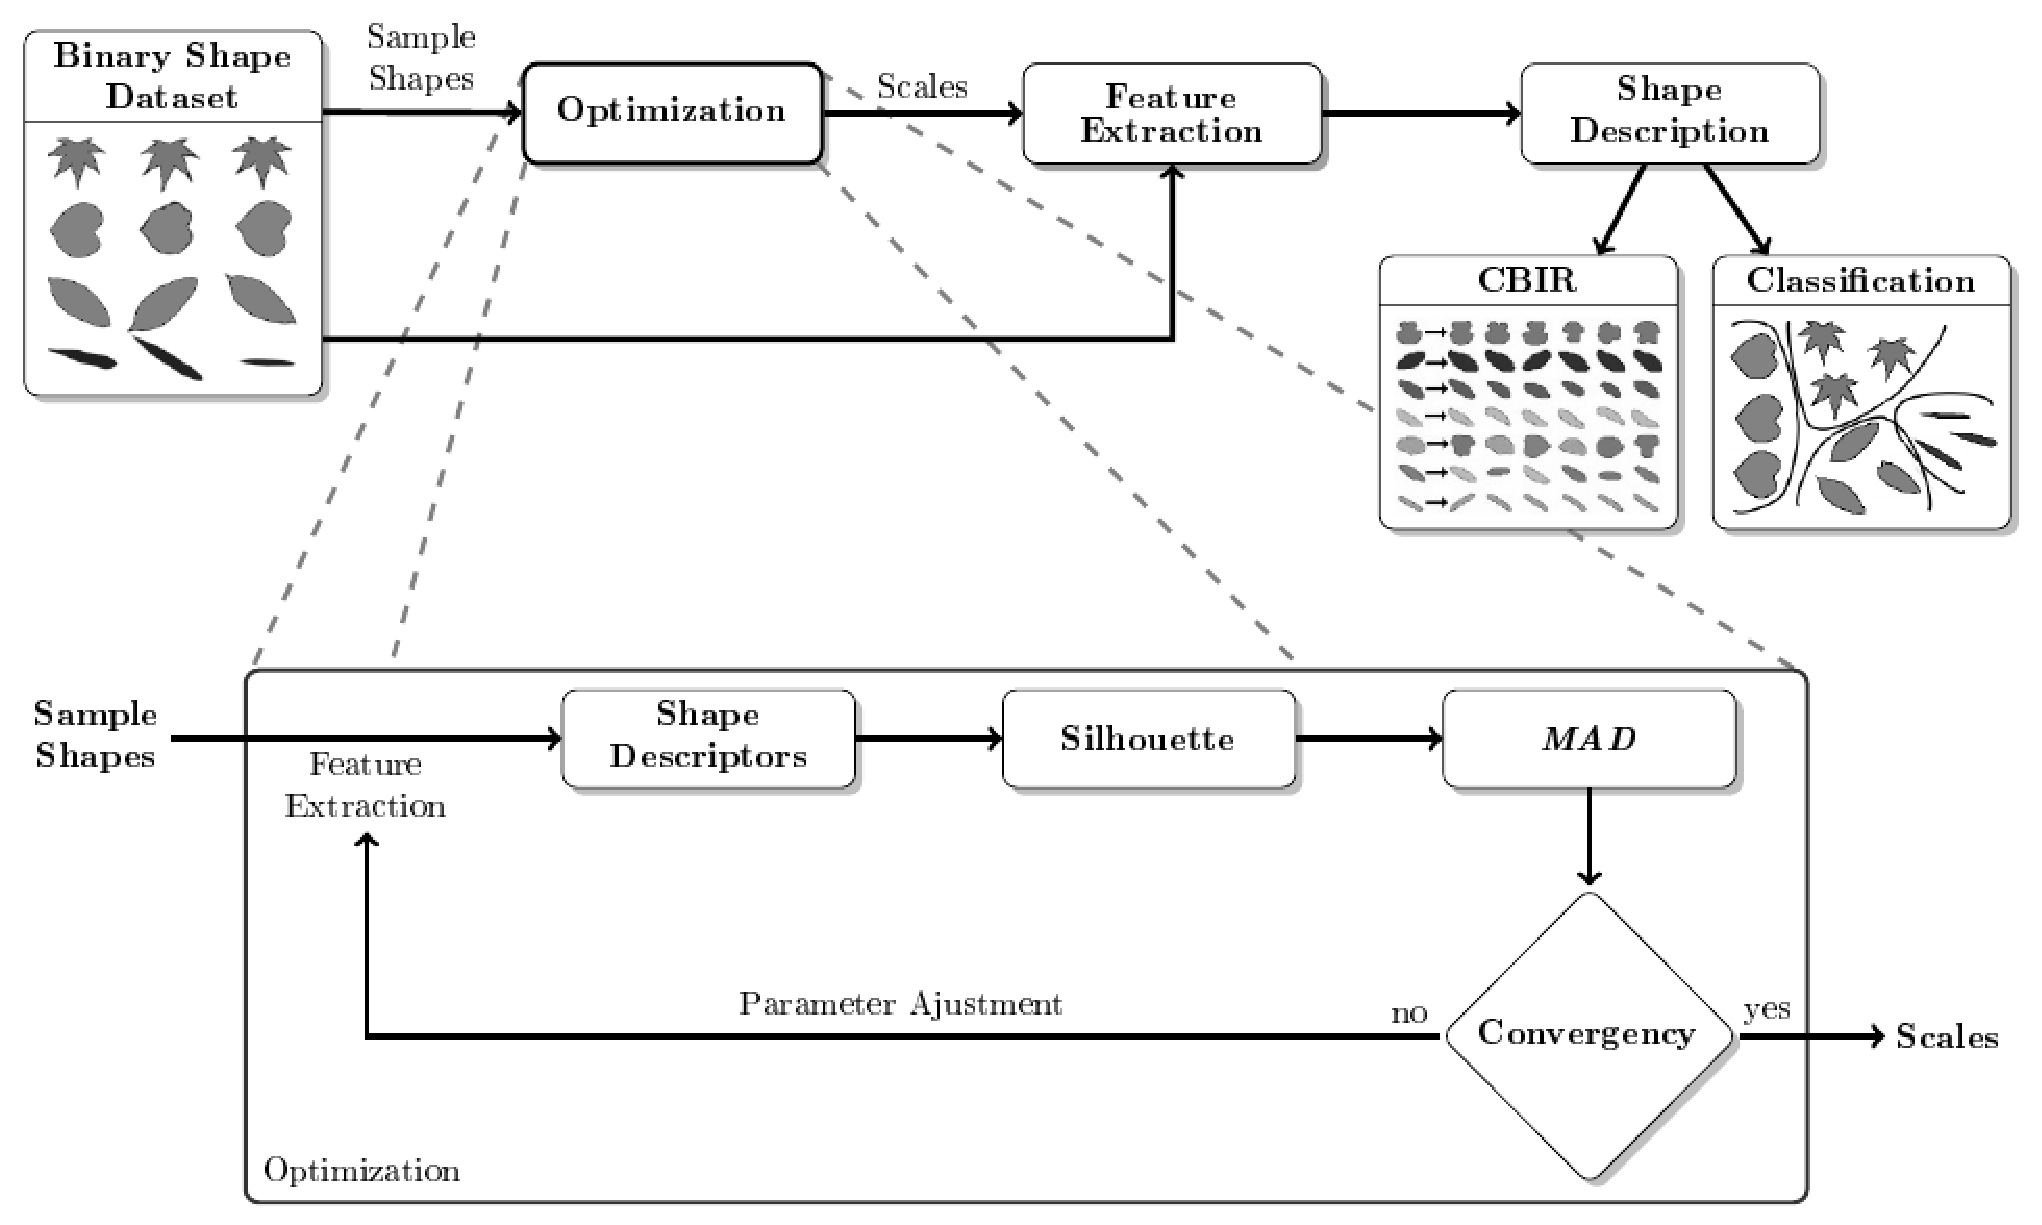
\includegraphics[width=\textwidth]{finalFlux.eps}
\end{figure*}

\noindent aonde $S = \{s_1,s_2,\cdots,s_L\}$ é o conjunto das \emph{silhouettes} calculadas para $L$ descritores de forma. Os operadores $|.|$  e {$mediana ( )$} retornam o valor absoluto e a mediana de um conjunto de valores, respectivamente.

A \textit{silhouette }\cite{Rousseeuw:1987} é uma medida de qualidade de agrupamentos que indica o grau de afinidade de uma amostra  a um agrupamento, levando em conta as distâncias médias entre classes e intra classes de um objeto $i$ atribuído a uma dada classe $A$. Logo, esta métrica é definida como 
\begin{equation}
s_i = \frac{b_i - a_i}{\max{(a_i,b_i)}} \in [-1,1],
\end{equation}

\noindent sendo $a_i$ a dissimilaridade média entre o objeto $i$ e os demais objetos pertencentes a mesma classe de $a_i$ e $b_i$ é a dissimilaridade média do objeto $i$ e a classe vizinha mais próxima de $i$, excluída sua própria classe. 

Essa métrica pode assumir valores no intervalo $[-1,1]$, sendo que valores negativos indicam que o grau de pertencimento de um objeto à classe que este fora atribuído é baixo. Já valores positivos indicam que o grau de pertencimento de um objeto à classe que este fora atribuído é alto. Um valor de silhouette próximo de zero indica que o objeto está na fronteira entre duas classes e que há, portanto, um grau de incerteza a respeito de qual classes este pertence.

Os valores da função objetivo $MAD$ assume valores no intervalo $[0,2]$. De forma análoga a silhouette, um valor igual a zero desta função indica que a estrutura dos clusters é perfeita, enquanto que valores próximos de $2$ indicam que a estrutura dos clusters é deficiente, com baixa similaridade entre os objetos de mesma classe ou alta similaridade entre os objetos de classes distintas.

%\section{Otimização}
Uma vez definida a função custo, o processo de otimização dos parâmetros descritor ajustará os mesmos ao problema em estudo. No caso da análise de formas de folhas, a otimização permite que os parâmetros, que minimizam a função objetivo ou função custo (\textit{MAD}),  incorporem nuances e detalhes do contorno das formas de folhas. O ajuste dos parâmetros ao problema em questão deverá melhorar as taxas de classificação e recuperação de formas de folhas de plantas. Vale destacar que a metodologia é versátil pois é ajustável a outras aplicações e portanto, suporta a definição de uma outra função objetivo. A Figura  \ref{fig:Avaliacao} ilustra, em detalhes, como se dá o ajuste dos parâmetros do descritor multiescala dentro da metodologia proposta, aplicada a um problema de análise de formas. Primeiramente, é amostrado na base de folhas um subconjunto das formas para, em seguida, realizar o procedimento de otimização e encontrar o melhor conjunto de parâmetros de escala  $\boldsymbol{\sigma}_{otim} = (\sigma_1,\:\sigma_2,\:\cdots,\:\sigma_k)$ do descritor NMBE que minimize a função custo da Equação \ref{eq:mad}. Então, utilizando-se as escalas encontradas realiza-se, com o descritor multiescala, a extração de características de toda a base de folhas e, em seguida, a avaliação de desempenho do mesmo.

\section{Avaliação do descritor}

O desempenho do descritor é avaliado neste trabalho qualitativamente e quantitativamente. Na avaliação qualitativa dois algoritmos de visualização de dados são utilizados: o mapa auto-organizável de Kohonen \cite{Kohonen:2001} e o \textit{escalonamento multidimensional} \cite{cox:2000}. Na avaliação quantitativa são analisadas as métricas de avaliação Precisão e Revocação, obtidas em experimentos de classificação supervisionada, a métrica \textit{Bulls-eye} \citeonline{Ling:2007:SCU:1191552.1191806}, classicamente utilizada na comparação de descritores em recuperação de formas (CBIR) e a medida de avaliação de agrupamentos silhouette \cite{Rousseeuw:1987}. 

Para fins de comparação,  as avaliações de desempenho qualitativa e quantitativa foram realizadas com as versões dos descritores otimizados com o método proposto e não otimizados, seja por escolha aleatória dos parâmetros ou por meio de ajuste apresentado em \cite{Costa:1997}.

\subsection{Visualização dos dados}

Algoritmos de visualização de dados produzem projeções bidimensionais das descrições das formas da base de folhas, provendo uma representação gráfica que possibilita a análise da qualidade dos agrupamentos. Assim, consegue-se inferir o quão eficaz o descritor é em organizar espacialmente as formas. Os métodos de visualização empregados neste trabalho são o mapa auto-organizável de Kohonen \cite{Kohonen:2001} e o \textit{escalonamento multidimensional (MDS)} \cite{cox:2000}.

As projeções \textit{MDS} da Figura \ref{fig:optimization_result} ilustram como os agrupamentos evoluem à medida que o algoritmo DE busca os parâmetros otimizados do descritor (NMBE). As amostras de formas exibidas pertencem à base Kimia-99 \cite{Sebastian:2004}, a qual contém $99$ imagens. Neste trabalho aplicamos técnicas de aprendizagem (\textit{manifold learning}) para produzir as projeções MDS do descritor NMBE otimizado utilizando o algoritmo DE.  A Figura \ref{fig:optimization_result} demonstra que à medida que os valores de MAD decrescem, as distâncias entre as classes aumentam e consequentemente os agrupamentos das classes se tornam mais evidentes. Nesta imagem, quando o método de otimização converge, ou seja MAD alcança o menor valor,   os únicos agrupamentos que não estão bem separados são aqueles relacionados às formas de animais quadrúpedes e de mãos. 

\begin{figure}[t]
\caption{\label{fig:optimization_result} Projeções do escalonamento multidimensional das formas da base Kimia-99 \citeonline{Sebastian:2004}. As imagens mostram como os agrupamentos evoluem ao longo do processo de otimização (DE), assim como os valores de MAD e $R^2$.}
\centering
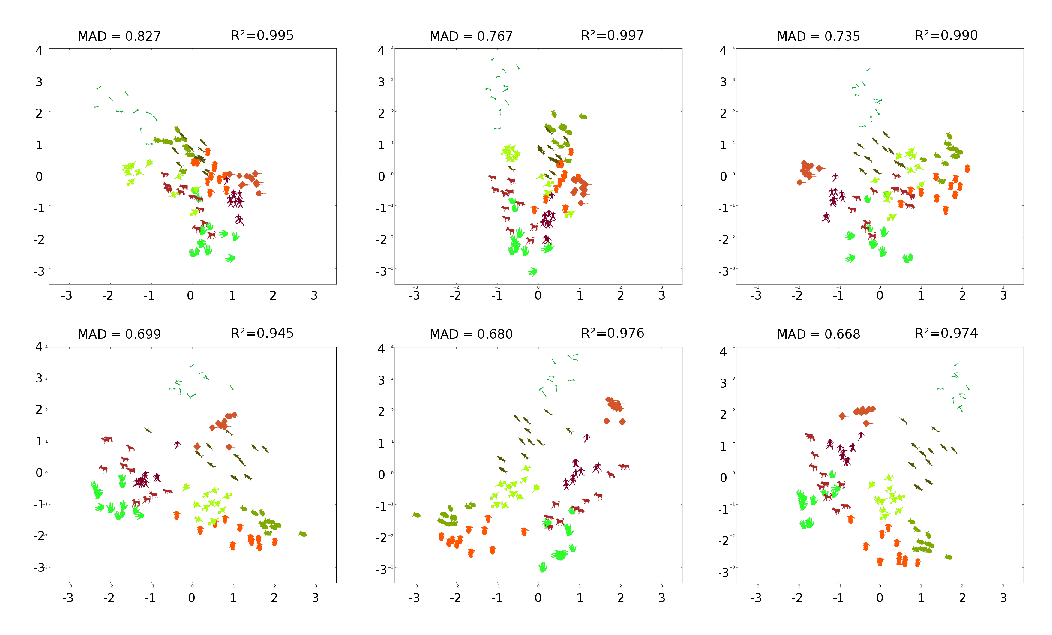
\includegraphics[width = \textwidth]{fig4.eps}
\end{figure}

\begin{figure}[!ht]
\caption{\label{fig:projkimia99} Matrizes-U para as formas da base MPEG7 CE-Shape-1.}
\centering
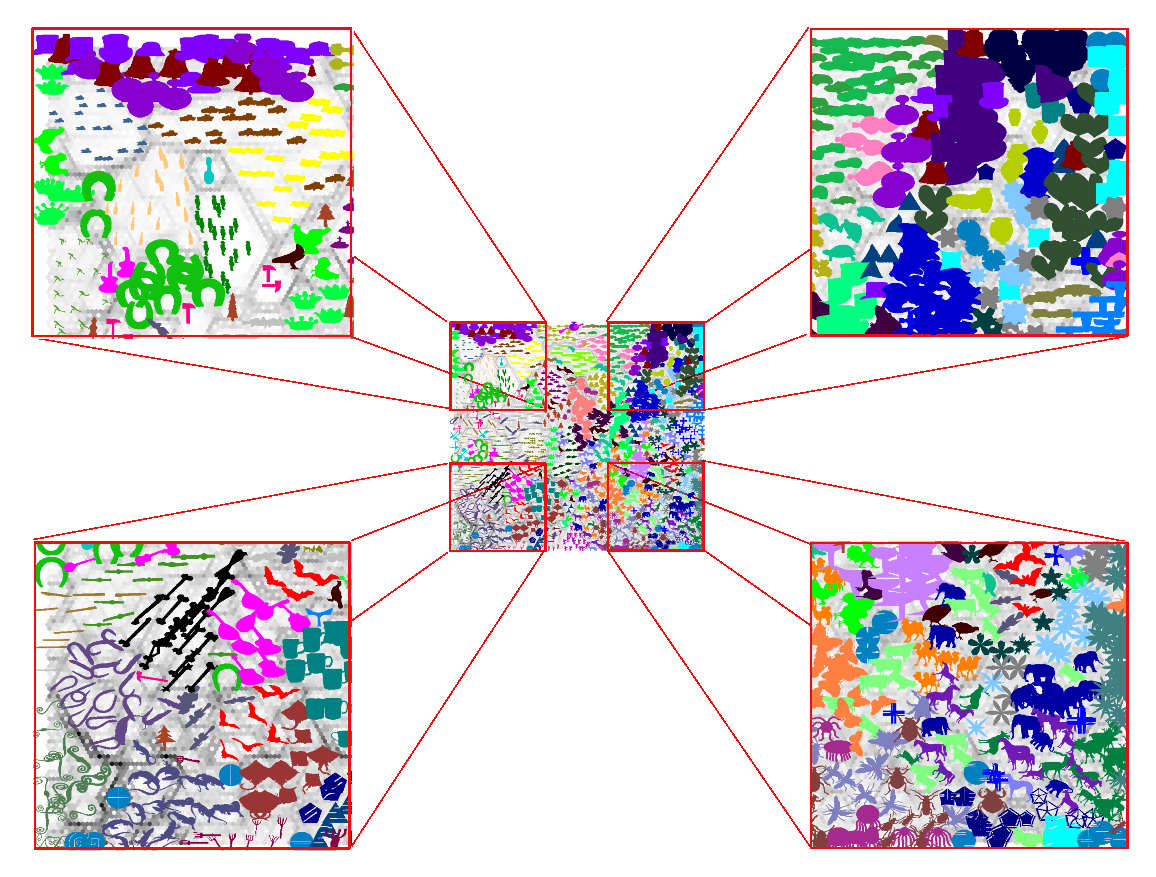
\includegraphics[width=\textwidth]{fig3.eps}
\end{figure}

\subsection{Recuperação de formas (CBIR)}

Foram realizados experimentos de recuperação de imagens pelo conteúdo visando avaliar o desempenho dos descritores de formas e das medidas de similaridade estudadas neste trabalho. As metodologias utilizadas nesses experimentos são as mesmas encontradas em diversos trabalhos de recuperação de formas da literatura.

Foram realizados experimentos em duas bases de imagens de formas binárias: a Kimia, de 99 formas, e a MPEG-7 CE-Shape-1 de 1400 formas. Ambas as bases estão apresentadas no Apêndice deste trabalho.

A  Figura \ref{fig:metodo_cbir} ilustra a metodologia dos experimentos de recuperação de formas.  Primeiramente realiza-se a extração de características das formas da base de imagens de formas binárias com o método de descrição sob avaliação. O mesmo processo de extração de características é aplicado a imagem de uma forma de consulta. Esse processo resulta numa base de dados com os vetores de características associados às formas utilizadas no experimento. 

Com a medida de similaridade avalia-se o grau de correspondência existente entre o vetor de características da forma de consulta e os vetores associados a cada uma das formas da base. Tem-se assim como resultado uma lista de imagens recuperadas em ordem decrescente de similaridade à forma de consulta. Todo esse processo é realizado repetidamente tomando-se cada forma da base de imagens como forma de consulta e recuperando-se as demais.

\begin{figure}[h!]
  \caption{\label{fig:metodo_cbir} Metodologia empregada para os experimentos de recuperação de formas pelo conteúdo.}
  \centering
  \includegraphics[width=0.55\textwidth]{Metodologia1.jpg}
\end{figure}

Na avaliação do desempenho dos experimentos duas medidas são utilizadas: o número total de acertos por posição recuperada e a medida bull-eyes.

A primeira medida consiste no número total de ocorrências de formas da mesma classe que a forma de consulta em cada posição recuperada.  Em diversos trabalhos de recuperação de formas pelo conteúdo o número total de acertos por posição recuperada é calculado para a base Kimia-99 \cite{Bernier:2003}. Tendo esta base 99 formas, igualmente distribuídas em 9 classes, são realizadas 99 recuperações das 11 formas mais similares à imagem de consulta. Como resultado espera-se obter um total de 99 formas recuperadas corretamente para cada posição recuperada.

A medida Bulls-eye também é utilizada na literatura para a comparação de diferentes métodos de recuperação de formas. Essa medida é calculada para a base MPEG-7 CE-Shape-1 da seguinte maneira: tomando-se cada forma dessa base de imagens como elemento de consulta, contabiliza-se o número de recuperações pertencentes a mesma classe da forma de consulta dentre as $40$ primeiras posições recuperadas. Como resultado calcula-se a percentagem da quantidade máxima de recuperações corretas possíveis de se alcançar, sendo esta última quantidade $28000 = 1400\text{ formas} \times 20\text{ recuperações corretas poro forma}$. 

\subsection{Classificação supervisionada}

\begin{figure*}[]
\caption{\label{fig:Classific}
Metodologia de classificação para avaliação de desempenho do descritor otimizado pelo método proposto exibido na Figura.  \ref{fig:Avaliacao}} 
\centering
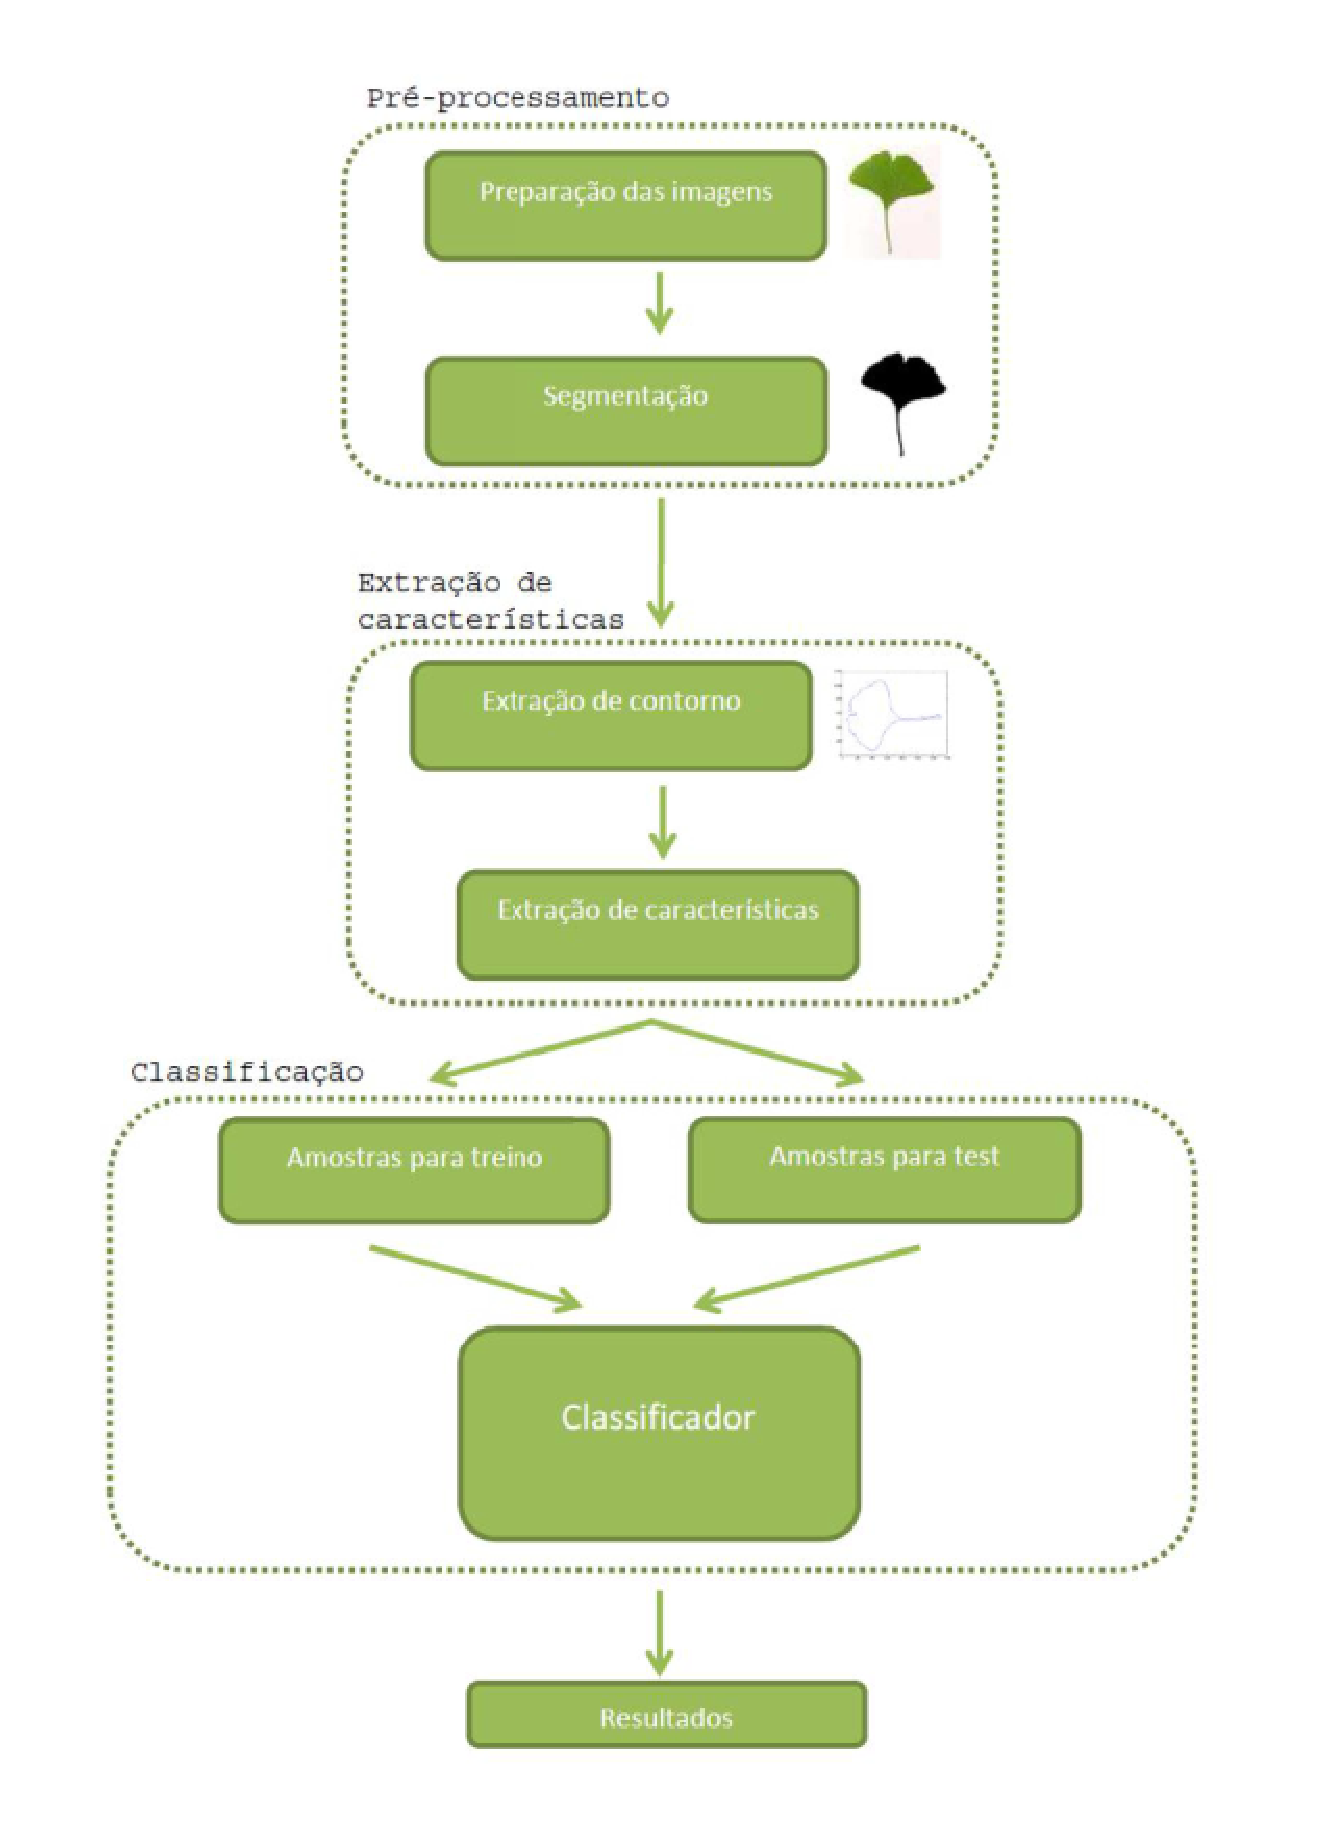
\includegraphics[width=0.7\textwidth]{fig_metodo_classifica_folhas.eps}
\end{figure*}

O procedimento adotado para avaliar o desempenho do descritor multiescala em classificação supervisionada está ilustrado na Figura \ref{fig:Classific}. A etapa de pré-processamento consiste na segmentação das imagens das formas. Essa etapa só se aplica para a base de folhas Flavia, aonde um método  de segmentação por limiar \cite{Gonzalez:2006} foi empregado. Para as formas das bases MPEG7-CE e Kimia-99, esta etapa não é necessária, pois as formas destas bases estão disponíveis já binarizadas.

Após a extração de características das formas, os descritores obtidos (vetores de características) são divididos em grupos de amostras de teste/treino pelo método de validação cruzada K-Fold (K = 10) \cite{Webb:2002}. Então, os descritores são transformados pelo discriminante linear de Fisher \cite{Webb:2002}, para melhorar a separação inter classes e a coesão intra classe, e em seguida, pela análise das componentes principais (PCA) para descorrelacioná-los. Cabe aqui salientar que as matrizes dessas transformações são obtidas apenas considerando as amostras de treino.

A etapa de classificação utiliza os classificadores Naive Bayes (NB) \cite{Fukunaga:1990}, \emph{K}-vizinhos próximos (Knn, $K = 5$) \cite{Fukunaga:1990,Webb:2002},  o discriminante linear de Fisher (LDA) \cite{Webb:2002} e o discriminante quadrático (QDA) \cite{Fukunaga:1990}. Para cada classificador foram realizadas $100$ execuções da validação cruzada, tendo como resultado os valores médios e os desvios da precisão e revocação obtidos nesses experimentos.  As medidas clássicas de precisão e revocação são empregadas na avaliação do desempenho de descritores em experimentos de classificação supervisionada.


\subsection{Avaliação quantitativa de agrupamentos}

A \textit{silhouette} média por classe avalia tanto a coesão como a separação das classes através da distância entre os vetores de características.




%A avaliação de similaridade entre formas a partir de medidas de divergência requer que as informações das assinaturas, abordadas na Seção \ref{sec:Assinatura} do Capítulo \ref{chap:contour}, sejam tratadas como variáveis aleatórias e que suas distribuições de probabilidade sejam estimadas. 

%A  Figura \ref{fig:metodo_distancia} ilustra como divergentes podem ser aplicados na avaliação da similaridade entre duas formas A e B. No método em questão, as distribuições de probabilidade de quatro assinaturas distintas dos contornos das formas são estimadas, através de histogramas, para em seguida se calcular as medidas de divergência. Uma medida de similaridade é então obtida  a partir da média ponderada das medidas de divergência.

\begin{comment}
\subsection{Visualização de dados}

A Figura \ref{fig:metodo_4} ilustra o método que empregamos na avaliação da capacidade discriminativa dos descritores de formas através das técnicas de visualização dos dados apresentadas.

\begin{figure}[h!]
  \caption{\label{fig:metodo_4} Método de avaliação de descritores multiescala do contorno de formas. (a) Base de imagens. (b) Extração de características. (c) Descritores de formas. (d) Análise de similaridade a partir da matriz-U. (e) Avaliação de agrupamentos a partir da medida silhouette.}
  \centering
  \includegraphics[width=\textwidth]{metodo_v4.png}
\end{figure}

O primeiro passo consiste em realizar a extração de características num conjunto de formas binárias rotuladas (Figura \ref{fig:metodo_4}a e Figura \ref{fig:metodo_4}b) com o método de descrição sob análise. Como resultado temos um conjunto de descritores, ou vetores de características, das referidas formas (Figura \ref{fig:metodo_4}c). 

A avaliação de qualidade dos descritores se dá qualitativamente e quantitativamente. Na avaliação qualitativa (Figura \ref{fig:metodo_4}d) utilizamos a rede auto-organizável de Kohonen para obtenção da matriz de distâncias unificada, ou matriz-U. Essa última é empregada como ferramenta de visualização dos dados, o que possibilita identificar como o método de descrição sob avaliação agrupa as formas. 

Na avaliação quantitativa (Figura \ref{fig:metodo_4}e) utilizamos os rótulos e os vetores de características das formas para calculamos a medida de avaliação de agrupamentos \emph{Silhouette} \cite{Rousseeuw:1987}. Valores médios dessa medida, por classe de formas, indica a habilidade dos descritores em discriminar formas que pertençam a classes distintas e de agrupar formas que pertençam a uma mesma classe.
\end{comment}

\begin{comment}
Although the curvature signal is a sensitive signature to local features of the shape contour, such as concavity and spatial location of salient points, its low noise immunity limits it for shape description application. Thus, it is recommended to smooth  the contour before calculating the curvature signal in order to yield a more robust representation, albeit losing information \citep{Cesar:1996}. A usual smoothing strategy is the discrete convolution of $z[n]$ with a Gaussian kernel, as follows

\begin{equation}
z_{\sigma}[n] = \sum_{i=1}^{N}z[i]g_{\sigma}[n-i],
\label{eq:zsigma}
\end{equation}

\noindent where $g_{\sigma}[n]$ is a Gaussian kernel filter and
$\sigma$ stands for the scale parameter for smoothing control. The Gaussian filter $g_{\sigma}[n]$ is given by\\ 

\begin{equation}
g_{\sigma}[n] = \frac{1}{\sigma\sqrt{2\pi}}e^{-n^{2}/2\sigma^{2}}. 
\end{equation}


It is well-known that this filtering process modifies the amplitude of the respective spectral representation of the contour in such a way that the contour tends to shrink as the kernel scale parameter decreases \citep{Cesar:1996,Costa:1997}. One strategy to avoid such effect is to normalize the smoothed contour as

\begin{equation}
\breve{z}_{\sigma}[n] = \frac{P}{P_{\sigma}}z_{\sigma}[n],
\end{equation}

\noindent where $P$ and $P_{\sigma}$ are the perimeters of the non-smoothed and smoothed contours, respectively.

By replacing $k[n]$ by $k_{\sigma}[n]$ and $z[n]$ by $\breve{z}_{\sigma} [n]$ in equations \ref{eq:ebe} and \ref{eq:kn}, and calculating these equations for $M$ different smoothing scale factors  $\sigma = (\sigma_{1}\text{, }\sigma_{2}\text{, }\ldots\text{ , }\sigma_{M})$, we obtain a multiscale representation of the bending energy given by:

\begin{equation}
NMBE = (\log{E_{\sigma_{1}}}\text{, }\log{E_{\sigma_{2}}}\text{, }\ldots \text{ , }\log{E_{\sigma_{M}}}).
\label{eq:nmbe}
\end{equation}
\end{comment}


%Os descritores entropia multiescala, apresentado no Capítulo \ref{chap:FUNDA}, e a energia de dobramento multiescala requerem o ajuste dos seguintes parâmetros: o número e os valores dos fatores de escala utilizados na representação das formas. Esse capítulo apresenta um método robusto e versátil para o ajuste desses parâmetros para customizar esses descritores em aplicações de classificação supervisionada e não supervisionada.   
